\documentclass[a4paper,12pt]{article}
\usepackage{graphicx}
\usepackage{hyperref}
\usepackage{amsmath}
\usepackage{times}
\usepackage{xcolor}
\usepackage{amsfonts}
\usepackage{garamondx}
\usepackage{framed}  %This is to use the shaded environment
\usepackage{titlesec}
\usepackage{upquote}



\titlespacing*{\section}
{0pt}{5.5ex plus 1ex minus .2ex}{4.3ex plus .2ex}
\titlespacing*{\subsection}
{0pt}{5.5ex plus 1ex minus .2ex}{4.3ex plus .2ex}

\usepackage{titling}
\setlength{\droptitle}{-8em} 


\textwidth=6.2in
\textheight=8.5in
%\parskip=.3cm
\oddsidemargin=.1in
\evensidemargin=.1in
\headheight=-.3in
\setlength{\parindent}{0pt}



% \renewcommand{\baselinestretch}{1} 
% \setlength{\parskip}{\baselineskip}
% \setlength{\parindent}{0pt}
% \setlength{\marginparwidth}{2.5cm}


\newcommand{\scscst}{\scriptscriptstyle}
\newcommand{\scst}{\scriptstyle}
\newcommand{\Robject}[1]{{\code{#1}}}
\newcommand{\Rfunction}[1]{{\code{#1}}}
\newcommand{\Rclass}[1]{\textit{#1}}
\newcommand{\Rpackage}[1]{\textit{#1}}
\newcommand{\Rexpression}[1]{\code{#1}}
\newcommand{\Rmethod}[1]{{\code{#1}}}
\newcommand{\Rfunarg}[1]{{\code{#1}}}

\newcommand\boldblue[1]{\textcolor{blue}{\textbf{#1}}}
\newcommand\code[1]{\textcolor{red}{\texttt{#1}}}

\usepackage{Sweave}
\begin{document}
\Sconcordance{concordance:1_Stats_Course_Notes-knitr.tex:1_Stats_Course_Notes-knitr.Rnw:%
1 50 1 1 0 5 1 1 7 13 1 1 9 1 1 1 7 160 1 1 5 9 0 1 2 5 1 1 2 1 0 2 1 %
13 0 1 2 8 1 1 2 1 0 1 3 4 0 1 2 3 1 1 4 1 1 1 4 7 0 1 2 8 1}

\definecolor{shadecolor}{gray}{0.95} %this is defining the color of the background in the shaded environment

%\SweaveOpts{concordance=TRUE}



%------------------------------------------------------------
\title{Using R as a Research Tool.\\
Part 2: R Markdown and basic statistics.}
%------------------------------------------------------------
\author{Dr Susan Johnston: \href{mailto:Susan.Johnston@ed.ac.uk}{Susan.Johnston@ed.ac.uk}  \\ \\
        Demonstrators: Gergana Daskalova, John Godlee. \\
        Hat-Tips to Kyle Dexter, The Coding Club and R4all.}
%\date{}











\maketitle

%\tableofcontents


%-------------------------------------------
\section {Introduction}
%-------------------------------------------

This practical will follow on from the previous practical in data manipulation and visualisation, exploring how to write reports in \boldblue{R} Markdown and how to conduct simple statistical tests in \boldblue{R}. By the end of the practical, you should be able to:

\begin{itemize}

\item Write, embed and render code and results into an HTML document.

\item Carry out basic statistics and visualisations, including:

\begin{itemize}

\item Linear regression with \code{lm()}
\item Chi-squared test with \code{chisq.test()}
\item 2-sample t-test with \code{t.test()}


\end{itemize}

\end{itemize}



%-------------------------------------------
\section {Writing reports with R Markdown.}
%-------------------------------------------


\boldblue{R} Markdown is a tool for writing, reproducible reports in \boldblue{R}. It can be used to produce documents with embedded code and figures in HTML, Word and PDF format, and can also be used to create webpages and slideshows. The current version of the \boldblue{R} Markdown Cheatsheet from RStudio has been attached to these course notes.

\subsection{Creating an R Markdown Document.}

Open RStudio and create a new markdown document by going to \textbf{File > New File > R Markdown...}. In the window, name your document, select \textbf{HTML} and click \textbf{OK}. RStudio should automatically create a template as in Figure \ref{fig:MarkdownTemplate} (if not - it is saved in the file \texttt{R\_Markdown\_Template.Rmd)}. \\

To render the document, click the button that says \textbf{Knit} (you may have to save it first). As you can see, it produces a formatted HTML document with embedded figures. \\

Another thing to note is the \textbf{Show document outline} in the top right corner of the window, which shows the document structure.

\begin{figure}[h]
	\centering 
	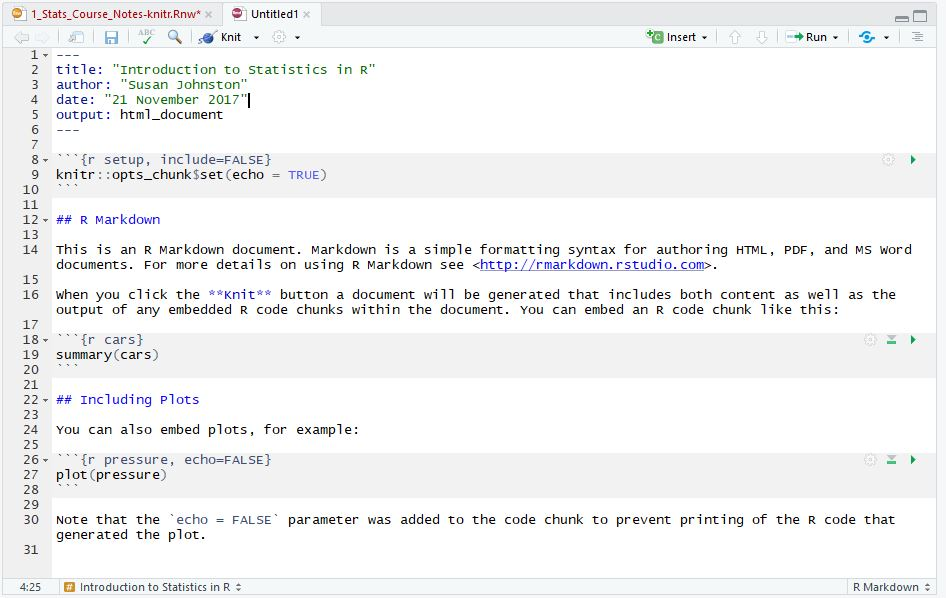
\includegraphics[width=0.9\textwidth]{figs/MarkdownTemplate.JPG}
	\caption{R Markdown Template.}
	\label{fig:MarkdownTemplate}
\end{figure} 

\subsection{Formatting an R Markdown Document.}

It is possible to carry out basic formatting, tables, headers, as well as adding tables, lists and external figures. See Part 3 of the \boldblue{R} Markdown CheatSheet from RStudio, which is attached to the back of this document. \\

\fbox{\begin{minipage}{36em}
\Large{\textbf{Exercise 1.}}

\normalsize
1. Create a new \boldblue{R} Markdown Script with the following header:\\


\texttt{---}\\
\texttt{title:} ``\texttt{Introduction to Statistics in R}''\\
\texttt{author:} ``\texttt{Your Name}''\\
\texttt{date:} ``\texttt{28 November 2017}'' \\
\texttt{output: html\_document} \\
\texttt{---} \\


Add some text to it and familiarise yourself with how to make \textit{italic}, \textbf{bold} and superscript text. Add headers for ``Introduction'', ``Linear regression'', ``Chi-squared test'' and ``Two-sample t-test``..
\end{minipage}}


\subsection{Embedding code in R Markdown.}

Code can be embedded into the document in two ways: \\

\textbf{Code Chunks:}
\begin{shaded}
\begin{verbatim}
```{r}
head(iris)
```
\end{verbatim}
\end{shaded}

Code chunks can be named, e.g. \verb!```{r iris}! \\

\textbf{Inline code:}
\begin{shaded}
\begin{verbatim}
Two plus two equals `r 2 + 2`.
\end{verbatim}
\end{shaded}

Which will print ``Two plus two equals 4.''. \\

There are also a number of display options for each chunk in section 5 of the cheat sheet. For example, 

\begin{shaded}
\begin{verbatim}
```{r echo = F, results = "hide", fig.width = 4, fig.height = 3}
head(iris)

library(ggplot2)
ggplot(iris, aes(x = Sepal.Length, y = Sepal.Width)) + geom_point()
```
\end{verbatim}
\end{shaded}

will show the code output and the figure (dimensions specified with \texttt{fig.width} and \texttt{fig.height}), but not the code itself (\texttt{echo = F}) or the console output (i.e. \texttt{head(iris)}; \texttt{results = "hide"}). \\

\subsection{Points to note.}

\begin{itemize}
\item Rendering the document with \textbf{Knit}, that R is opening and creating a new working environment. Each code chunk that is run is saved in the workspace - therefore, libraries and new objects created in a chunk will remain in the workspace for all subsequent chunks. 

\item It's good to put a chunk at the start loading the libraries and data.

\item Code in \boldblue{R} Markdown chunks can be run in the console as in the previous practical. The default option is to show the code output inline in the document. Some people like this, others don't: to switch this function on and off, go to \textbf{Global options > R Markdown >Show output inline for all Markdown documents} and select your preferred setup. 

\item \boldblue{R} Markdown documents are not flexible to errors - the code must be error free, or it will not render. 

\item Want to learn more? More detailed information on this can be found at the Coding Club tutorial at \url{https://ourcodingclub.github.io/2016/11/24/rmarkdown-1.html}.

\end{itemize}


\fbox{\begin{minipage}{36em}

For the rest of the practical, it is expected that you create an R Markdown document that contains text, code, graphs and inline reporting of results.
\end{minipage}}


%-------------------------------------------
\section{Basic statistics.}
%-------------------------------------------

Question > visualisation > statistic > render

%-------------------------------------------
\section{$\chi^{2}$ contingency table}
%-------------------------------------------

A $\chi ^{2}$ contingency table analyses count data, and looks at the association between two or more categorical variables. In this example, we will examine the differences in the frequency of red and black ladybirds (\textit{Adalia bipunctata}) in rural and industrial habitats. Our question is: are dark morphs more likely to reside in dark (industrial) backgrounds? The null hypothesis is that there is no association between ladybird colour morph and habitat type \footnote{The approach and dataset here is based on the example presented in the book ``Getting Started with R'' (2nd Edition, 2017) by Beckerman, Childs and Petchey (\url{http://www.r4all.org})}}. \\

Load the data file \texttt{ladybirds.csv} into R using \code{read.csv()} and examine it using \code{glimpse()} from the \code{dplyr} package.\\

\begin{shaded}
\begin{verbatim}
library(dplyr)

ladybirds <- read.csv("data/ladybirds.csv", header = T)
glimpse(ladybirds)
\end{verbatim}
\end{shaded}

\begin{Schunk}
\begin{Soutput}
Observations: 20
Variables: 4
$ Habitat      <fctr> Rural, Rural, Rural, Rural, Rural, Rural, Rural, Rura...
$ Site         <fctr> R1, R2, R3, R4, R5, R1, R2, R3, R4, R5, U1, U2, U3, U...
$ morph_colour <fctr> black, black, black, black, black, red, red, red, red...
$ number       <int> 10, 3, 4, 7, 6, 15, 18, 9, 12, 16, 32, 25, 25, 17, 16,...
\end{Soutput}
\end{Schunk}

There are multiple lines for each category, with the column number giving the count details. We ultimately want four numbers, corresponding to the 2 $\times$ 2 categories: red industrial, black industrial, red rural and black rural. \\

This can be done using the \code{dplyr} functions \code{group\_by()} amd \code{summarise()}.

\begin{shaded}
\begin{Schunk}
\begin{Sinput}
> totals <- group_by(ladybirds, Habitat, morph_colour)
> totals <- summarise(totals, total.number = sum(number))
> totals
\end{Sinput}
\begin{Soutput}
# A tibble: 4 x 3
# Groups:   Habitat [?]
     Habitat morph_colour total.number
      <fctr>       <fctr>        <int>
1 Industrial        black          115
2 Industrial          red           85
3      Rural        black           30
4      Rural          red           70
\end{Soutput}
\end{Schunk}
\end{shaded}


\subsection{Plot the data}

One visualisation for this type of data is a bar chart using \code{geom\_col()} in \code{ggplot2}.


\begin{shaded}
\begin{Schunk}
\begin{Sinput}
> library(ggplot2)
> ggplot(totals, aes(x = Habitat, y = total.number, fill = morph_colour)) +
+   geom_col() 
\end{Sinput}
\end{Schunk}
\end{shaded}

There are two edits we can make to this to improve the visualisation: to add \code{geom\_col(position = "dodge")} to place bars side by side, and also by changing the colours of the bars to black and red to match the colour of the morphs in real life (using \code{scale\_fill\_manual()}):


\begin{shaded}
\begin{Schunk}
\begin{Sinput}
> ggplot(totals, aes(x = Habitat, y = total.number, fill = morph_colour)) +
+   geom_col(position = "dodge") +
+   scale_fill_manual(values = c(black = "black", red = "red"))
\end{Sinput}
\end{Schunk}
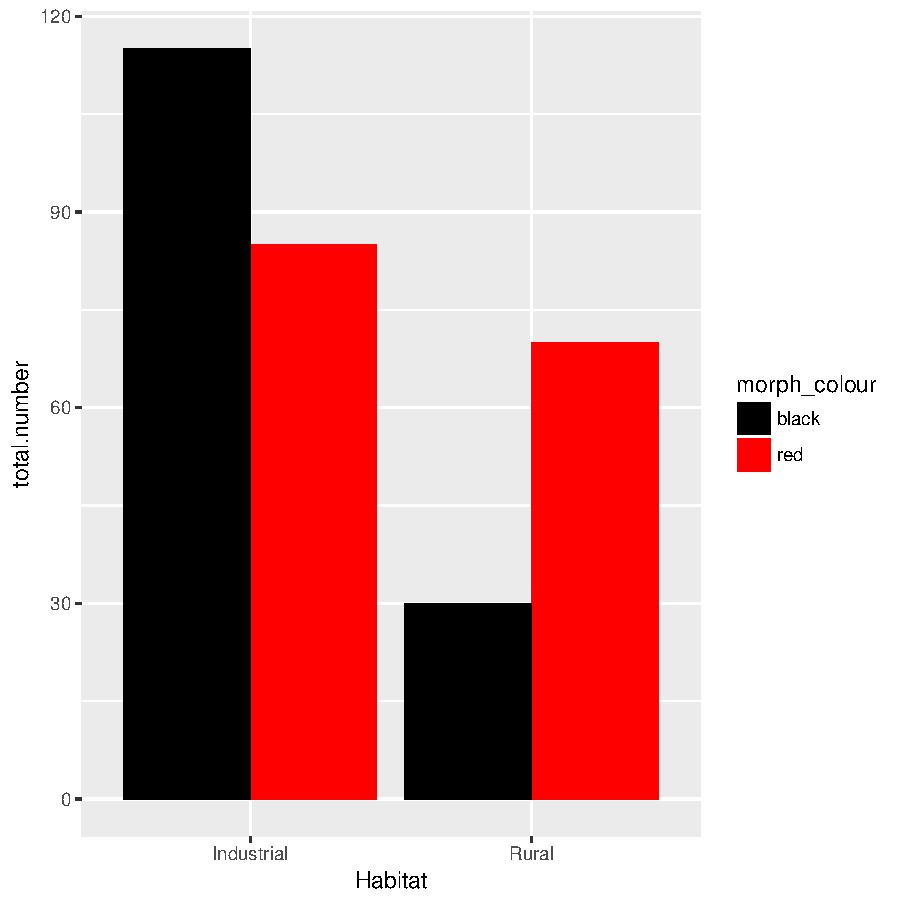
\includegraphics{1_Stats_Course_Notes-knitr-008}
\end{shaded}

\subsection{Test the hypothesis with \code{chisq.test()}.}

The $\chi^{2}$ is run using the function \code{chisq.test()}. As this is a 2 $\times$ 2 contingency test, we must convert the data into a matrix. Looking at the data \code{ladybirds}, a matrix can be made using the function \code{xtabs()}, which is similar to creating pivot table cross-tabulation in Excel:

\begin{shaded}
\begin{Schunk}
\begin{Sinput}
> lady.mat <- xtabs(number ~ Habitat + morph_colour, data = ladybirds)
> lady.mat
\end{Sinput}
\begin{Soutput}
            morph_colour
Habitat      black red
  Industrial   115  85
  Rural         30  70
\end{Soutput}
\end{Schunk}
\end{shaded}

Now run the test:

\begin{shaded}
\begin{Schunk}
\begin{Sinput}
> chisq.test(lady.mat)
\end{Sinput}
\begin{Soutput}
	Pearson's Chi-squared test with Yates' continuity correction

data:  lady.mat
X-squared = 19.103, df = 1, p-value = 1.239e-05
\end{Soutput}
\end{Schunk}
\end{shaded}


This provides a statistic indivating that there is a very small probability that the observed pattern arose by chance. Therefore, we can reject the null hypothesis.

We can extract more information from the statistic if we save the \code{chisq.test(ladymat)} as an object:

\begin{shaded}
\begin{Schunk}
\begin{Sinput}
> lady.chisq <- chisq.test(lady.mat)
\end{Sinput}
\end{Schunk}
\end{shaded}

Running \code{lady.chisq} gives the same output as before, but we can explore the object in detail using the \code{\$} notation:

\begin{shaded}
\begin{Schunk}
\begin{Sinput}
> names(lady.chisq)
\end{Sinput}
\begin{Soutput}
[1] "statistic" "parameter" "p.value"   "method"    "data.name" "observed" 
[7] "expected"  "residuals" "stdres"   
\end{Soutput}
\begin{Sinput}
> str(lady.chisq)
\end{Sinput}
\begin{Soutput}
List of 9
 $ statistic: Named num 19.1
  ..- attr(*, "names")= chr "X-squared"
 $ parameter: Named int 1
  ..- attr(*, "names")= chr "df"
 $ p.value  : num 1.24e-05
 $ method   : chr "Pearson's Chi-squared test with Yates' continuity correction"
 $ data.name: chr "lady.mat"
 $ observed : int [1:2, 1:2] 115 30 85 70
  ..- attr(*, "dimnames")=List of 2
  .. ..$ Habitat     : chr [1:2] "Industrial" "Rural"
  .. ..$ morph_colour: chr [1:2] "black" "red"
  ..- attr(*, "class")= chr [1:2] "xtabs" "table"
  ..- attr(*, "call")= language xtabs(formula = number ~ Habitat + morph_colour, data = ladybirds)
 $ expected : num [1:2, 1:2] 96.7 48.3 103.3 51.7
  ..- attr(*, "dimnames")=List of 2
  .. ..$ Habitat     : chr [1:2] "Industrial" "Rural"
  .. ..$ morph_colour: chr [1:2] "black" "red"
 $ residuals: xtabs [1:2, 1:2] 1.86 -2.64 -1.8 2.55
  ..- attr(*, "class")= chr [1:2] "xtabs" "table"
  ..- attr(*, "call")= language xtabs(formula = number ~ Habitat + morph_colour, data = ladybirds)
  ..- attr(*, "dimnames")=List of 2
  .. ..$ Habitat     : chr [1:2] "Industrial" "Rural"
  .. ..$ morph_colour: chr [1:2] "black" "red"
 $ stdres   : xtabs [1:2, 1:2] 4.49 -4.49 -4.49 4.49
  ..- attr(*, "class")= chr [1:2] "xtabs" "table"
  ..- attr(*, "call")= language xtabs(formula = number ~ Habitat + morph_colour, data = ladybirds)
  ..- attr(*, "dimnames")=List of 2
  .. ..$ Habitat     : chr [1:2] "Industrial" "Rural"
  .. ..$ morph_colour: chr [1:2] "black" "red"
 - attr(*, "class")= chr "htest"
\end{Soutput}
\begin{Sinput}
> lady.chisq$statistic
\end{Sinput}
\begin{Soutput}
X-squared 
 19.10289 
\end{Soutput}
\begin{Sinput}
> lady.chisq$p.value
\end{Sinput}
\begin{Soutput}
[1] 1.238571e-05
\end{Soutput}
\end{Schunk}
\end{shaded}

In the \boldblue{R} Markdown document, it is possible to quote statistics inline using the \verb!`r`! notation e.g. \verb!`r lady.chisq$statistic`! and \verb!`r lady.chisq$p.value`! will print the $\chi^{2}$ statistic and P value inline, respectively. \\


\fbox{\begin{minipage}{36em}
\Large{\textbf{Exercise 2.}}\\

\normalsize 
Create a short report in the \boldblue{R} Markdown document with an inline report of the test statistics and P-value. This can be done as follows:
\begin{enumerate}
\item Run a code chunk for loading and manipulating the ladybird data, and running the $\chi^{2}$ test that does not print the code or results to the compiled document (hint: define \code{echo} and \code{results} in the chunk options).
\item Write a few lines of text stating the hypothesis, the test statistic and interpretation. E.g. \textit{The null hypothesis is... Ladybird morphs are not equally distributed in the two habitats (Chi squared = ..., df = ..., P = ...), with black morphs being more frequent in.... (Figure 1)}
\item Run another code chunk to create a barplot for Figure 1.
\end{enumerate}

\end{minipage}}

%-------------------------------------------
\section{Two-sample t-test.}
%-------------------------------------------

\begin{Schunk}
\begin{Sinput}
> sepals <- read.csv("../data/iris.edited.csv", header = T)
> str(sepals)
\end{Sinput}
\begin{Soutput}
'data.frame':	100 obs. of  2 variables:
 $ Species     : Factor w/ 2 levels "versicolor","virginica": 1 1 1 1 1 1 1 1 1 1 ...
 $ Sepal.Length: num  7 6.4 6.9 5.5 6.5 5.7 6.3 4.9 6.6 5.2 ...
\end{Soutput}
\begin{Sinput}
> ggplot(sepals, aes(Species, Sepal.Length)) + geom_boxplot()
> ggplot(sepals, aes(Sepal.Length)) + 
+   geom_histogram(binwidth = 0.2) + 
+   facet_wrap(~Species, ncol = 1)
> t.test(Sepal.Length ~ Species, data = sepals)
\end{Sinput}
\begin{Soutput}
	Welch Two Sample t-test

data:  Sepal.Length by Species
t = -5.6292, df = 94.025, p-value = 1.866e-07
alternative hypothesis: true difference in means is not equal to 0
95 percent confidence interval:
 -0.8819731 -0.4220269
sample estimates:
mean in group versicolor  mean in group virginica 
                   5.936                    6.588 
\end{Soutput}
\begin{Sinput}
> 
\end{Sinput}
\end{Schunk}

%-------------------------------------------
\section{Linear regression.}
%-------------------------------------------




\end{document}

